\documentclass[twocolumn,11pt]{article}
\setlength{\textheight}{9truein}
\setlength{\topmargin}{-0.9truein}
\setlength{\parindent}{0pt}
\setlength{\parskip}{10pt}
\setlength{\columnsep}{.4in}

\usepackage{amsmath,amsfonts,amssymb,amsthm,bm,caption,calc,ifthen,graphicx,url,hyperref}

\begin{document}
\pagestyle{plain}
\onecolumn
ASTP720 
\newline Homework 2
\newline Will Wainwright
\newline Repository: \href{https://github.com/wjwainwright/ASTP720}{https://github.com/wjwainwright/ASTP720}

\section*{Writeup}
Writing the calculus library was pretty straightforward, and I haven't run into any issues with the methods in testing. That being said, I didn't really get to apply the integration methods in the later questions. As for the matrix library, that took a lot longer to complete. For the basic framework I chose to use Numpy 2d arrays so that I could use simpler algorithms for indexing and utilize Numpy methods. The addition and multiplication were relatively straightforward, but the later methods took the most time. I used recursion to create residual matrices and take the determinant until a 2x2 matrix was reached. I utilized the same residual matrix method for the inversion method. Finally, I create the lower and upper matrices that multiply to the original using the LU decomposition method, and then assert that the LU determinant is equal to the origional determinant to ensure that both methods work. Due to time constraints, I was not able to get to number 5, though I know how to do it. I would create a matrix system of equations using the coefficients in the given .dat file and invert the matrix to solve for the number densities $n_1$ through $n_9$. Below are the plots generated from number 2. As for number 4, most of my unit testing was done in the matrix.py file.

\begin{figure}[!h]
	\centering
	\noindent
	\makebox[\textwidth]{
      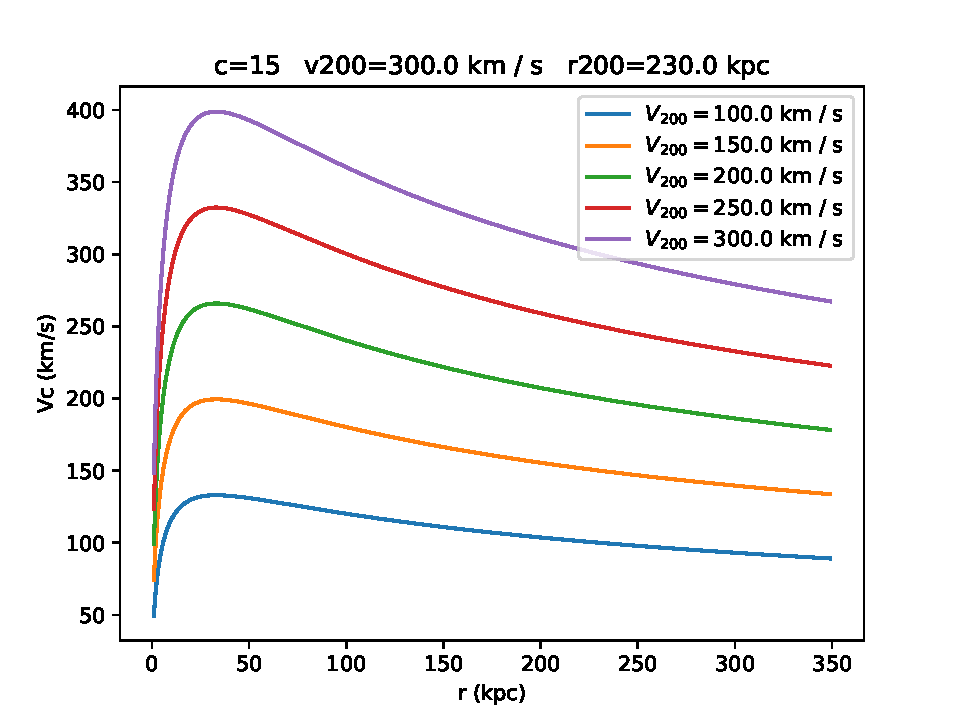
\includegraphics[width=4.5in]{Vc_r_15.pdf}}
      \caption{Decreasing the $V_{200}$ appears to shift the whole curve down and flatten the overall profile of the curve.}
\end{figure}
\begin{figure}[!h]
	\centering
	\noindent
	\makebox[\textwidth]{
      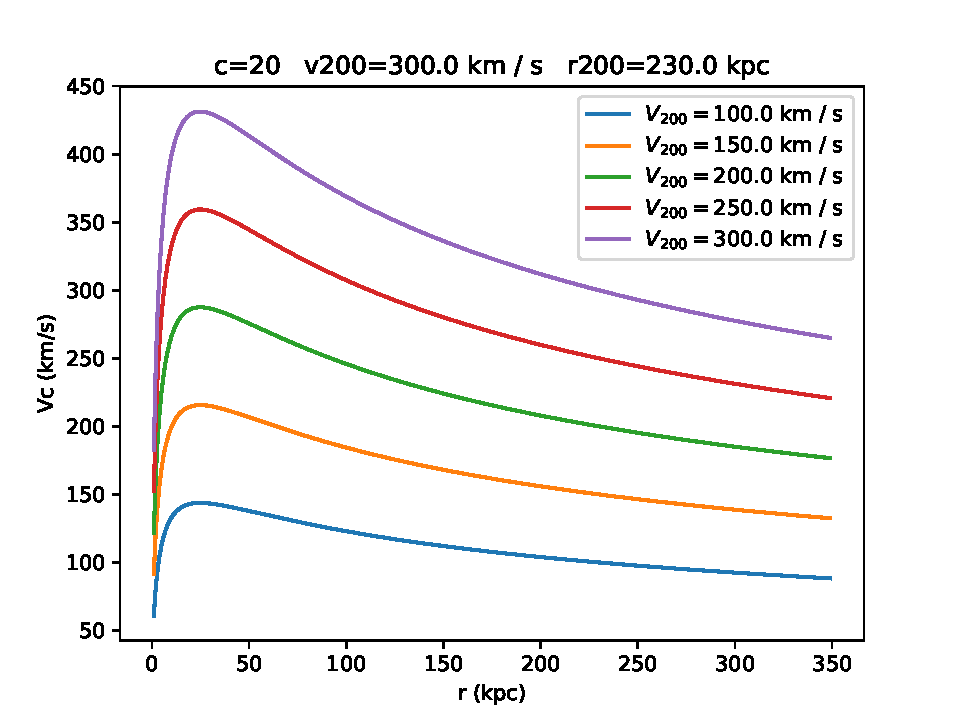
\includegraphics[width=4.5in]{Vc_r_20.pdf}}
      \caption{Increasing c and keeping $V_{200}$ constant appears to bring the peak of the curve to a higher $V_c$ value}
\end{figure}
\begin{figure}[!h]
	\centering
	\noindent
	\makebox[\textwidth]{
      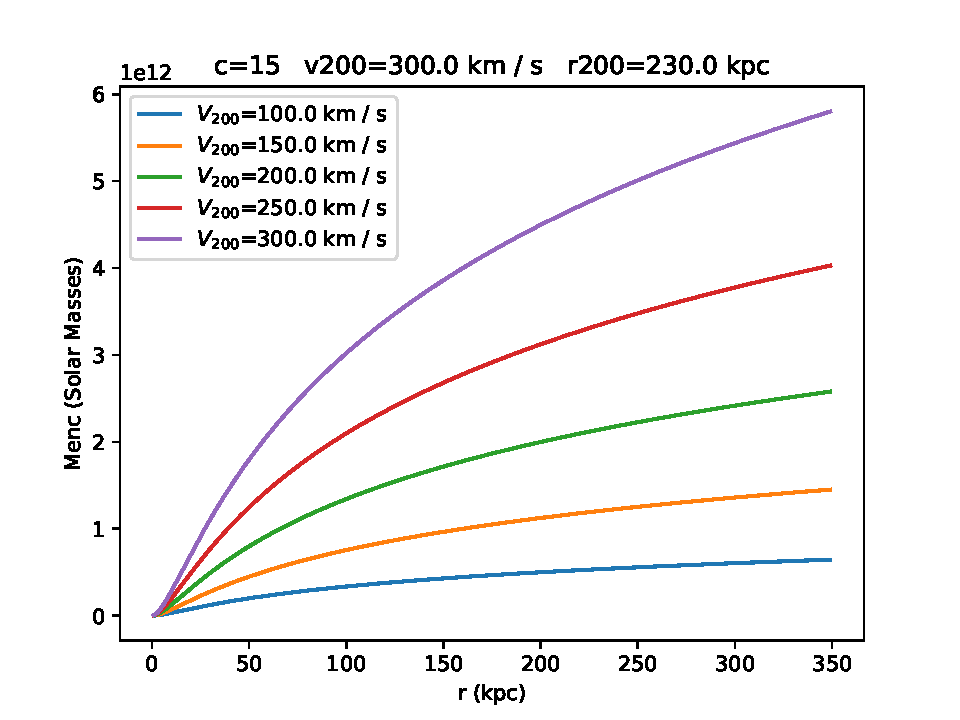
\includegraphics[width=4.5in]{Menc_r_15.pdf}}
      \caption{The mass enclosed as a function of radius changes quite drastically as a function of $V_{200}$.}
\end{figure}
\begin{figure}[!h]
	\centering
	\noindent
	\makebox[\textwidth]{
      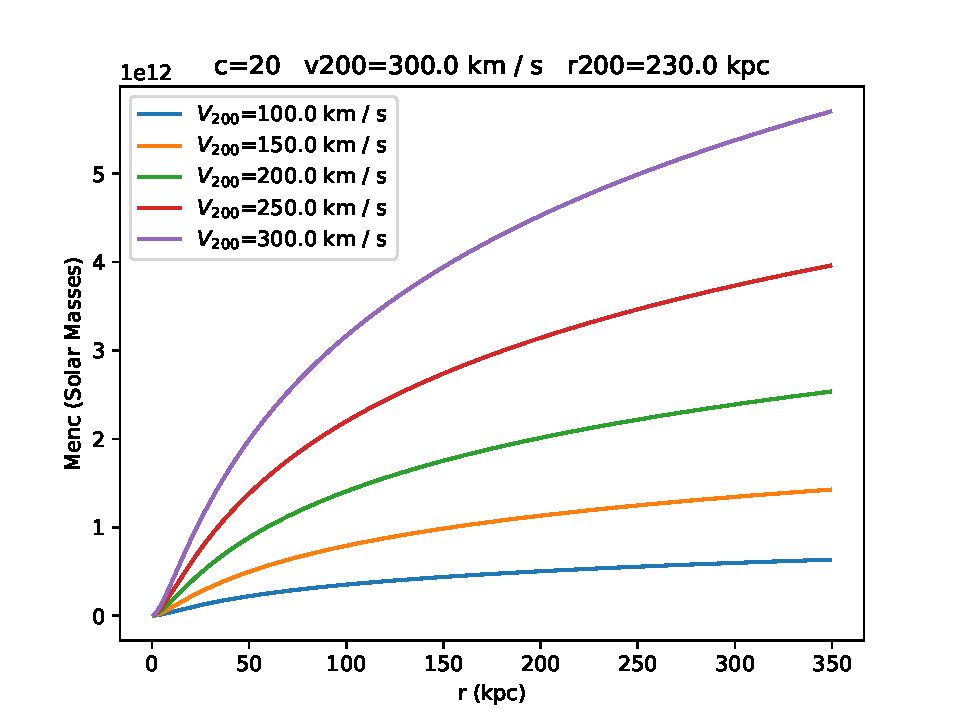
\includegraphics[width=4.5in]{Menc_r_20.pdf}}
      \caption{Interestingly, increasing c when compared to Figure 3 decreases the enclosed mass at the same $V_{200}$.}
\end{figure}
\begin{figure}[!h]
	\centering
	\noindent
	\makebox[\textwidth]{
      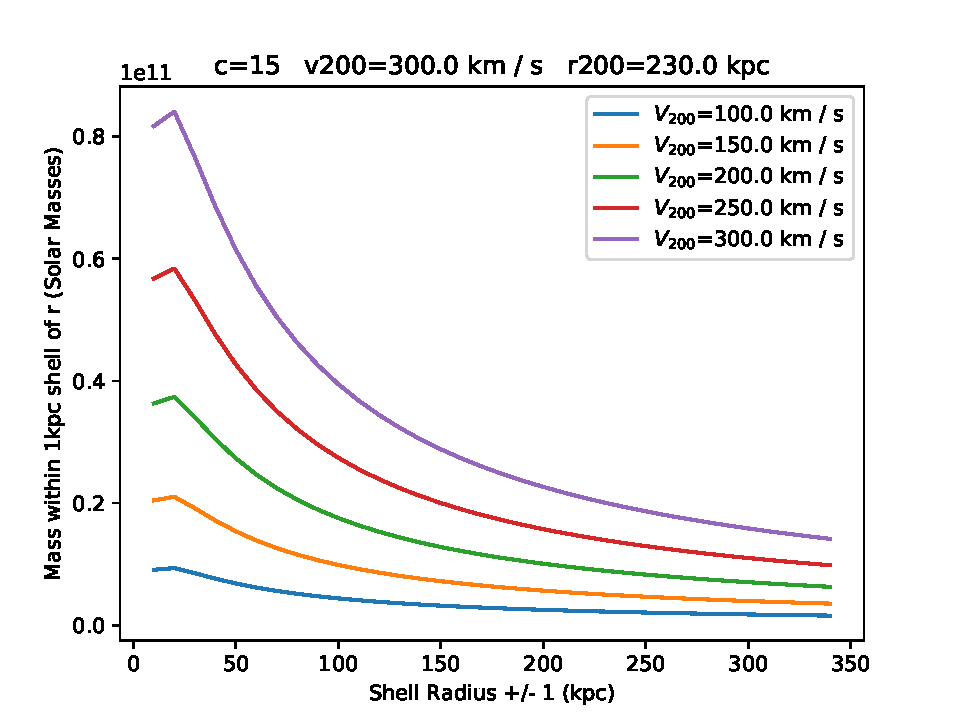
\includegraphics[width=4.5in]{Mass_shell_15.pdf}}
      \caption{The mass at a given shell decreased drastically from the center to around 100kpc and then plateaus. Decreasing $V_{200}$ causes it to plateau faster and start lower.}
\end{figure}
\begin{figure}[!h]
	\centering
	\noindent
	\makebox[\textwidth]{
      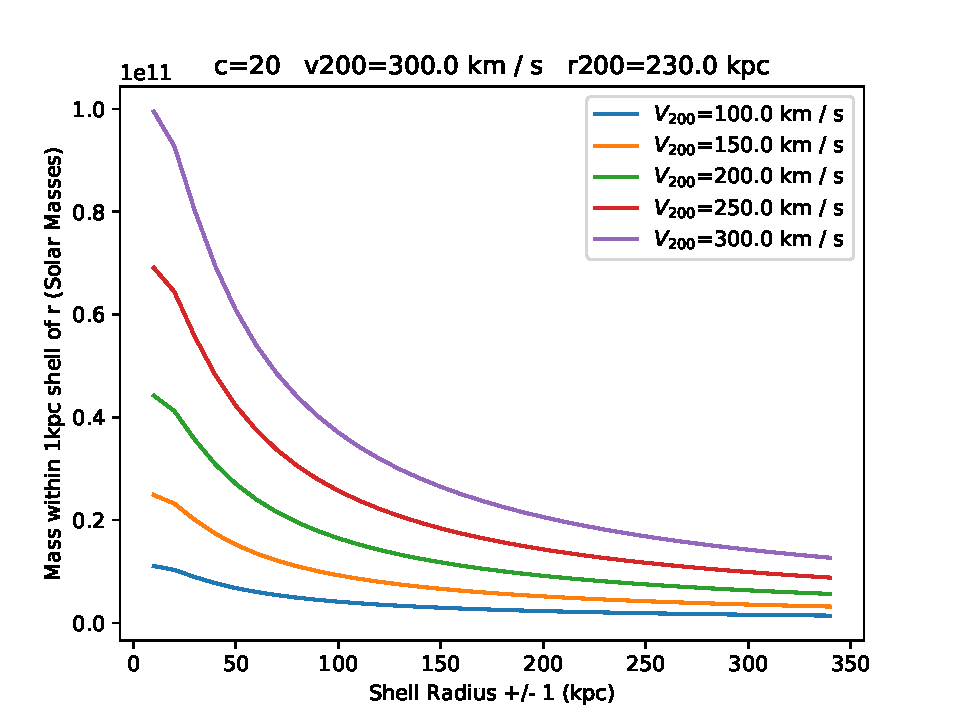
\includegraphics[width=4.5in]{Mass_shell_20.pdf}}
      \caption{Increasing c increases the initial mass but the plateau mass remains roughly the same.}
\end{figure}
\begin{figure}[!h]
	\centering
	\noindent
	\makebox[\textwidth]{
      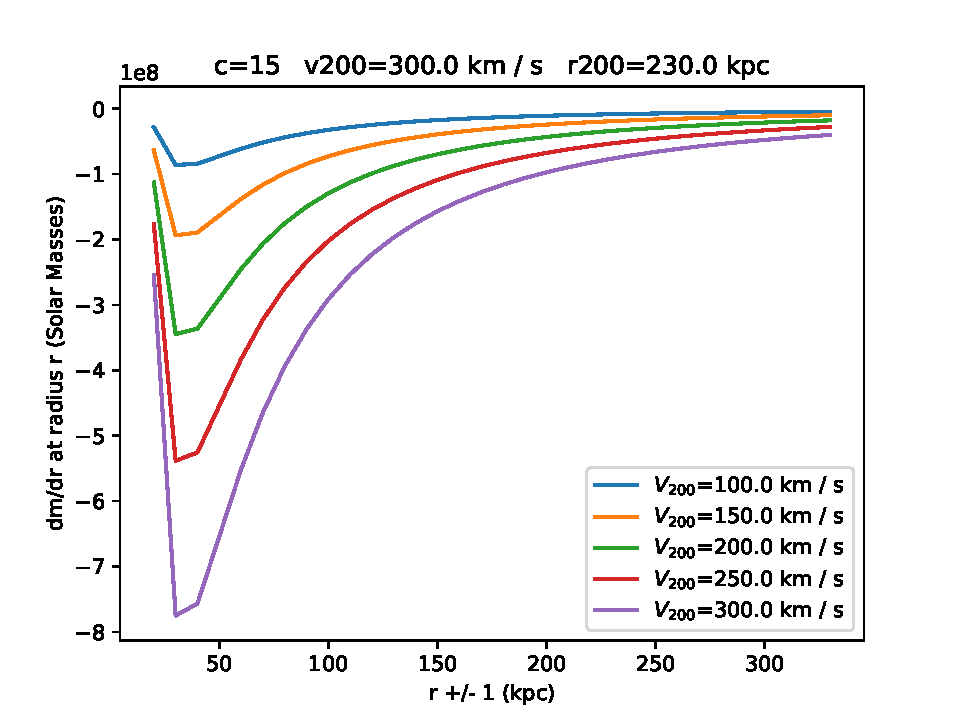
\includegraphics[width=4.5in]{dM_dR_15.pdf}}
      \caption{Obtained by taking the numerical derivative of the points making up the plot of mass enclosed within a given shell.}
\end{figure}
\begin{figure}[!h]
	\centering
	\noindent
	\makebox[\textwidth]{
      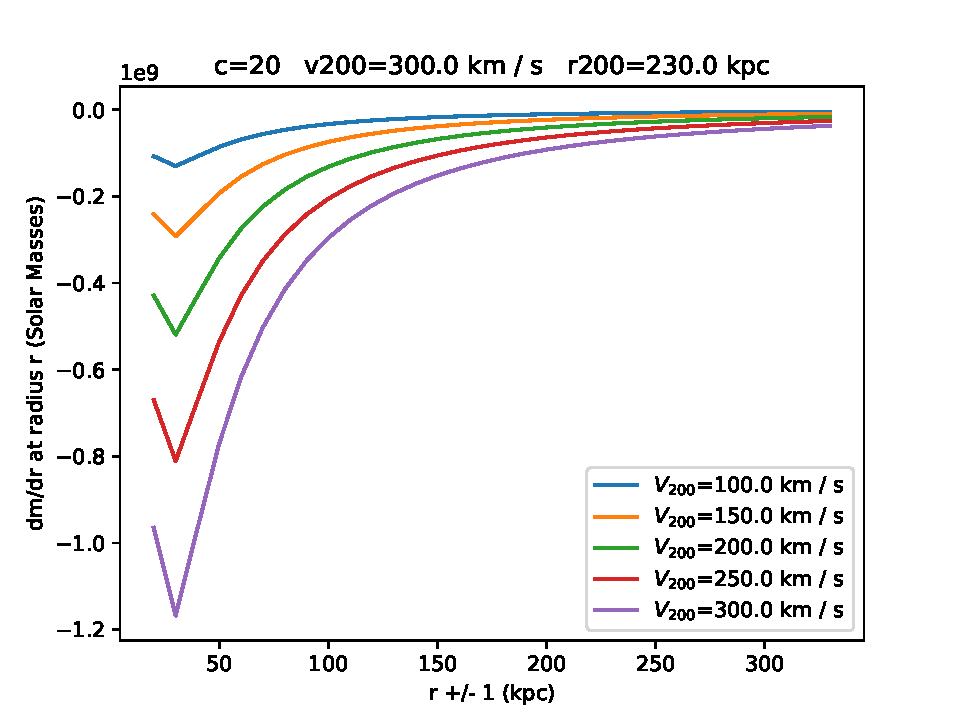
\includegraphics[width=4.5in]{dM_dR_20.pdf}}
      \caption{The initial points are shifted down with increasing c, but the plateau point of convergence remains similar.}
\end{figure}

\end{document}